\documentclass[11pt,t,usepdftitle=false,aspectratio=169]{beamer}
\usepackage{biblatex}
\usepackage{color}
\usepackage{amsmath}
\usepackage{algorithm}
\usepackage{algpseudocode}


\definecolor{green}{RGB}{0,220,0}
\definecolor{orange}{RGB}{240,220,0}
\definecolor{blue}{RGB}{0,0,255}
\definecolor{red}{RGB}{255,0,0}

\addbibresource{bibliography.bib}

\usetheme[nototalframenumber,foot,logo]{uibk}

%% information for the title page
\title[Resampling Detection - Finale Präsentation]{Resampling Detection}
\subtitle{Kirchner's Fast Detection Method - Forensische Analyse}

\author[Dominik Barbist, Lukas Egger]{Dominik Barbist, Lukas Egger \\ \vspace{0.5em}}
\footertext{Digitale Forensik mit Bild- und Videodaten - Finale Präsentation}
\date{\today}

\headerimage{3}

\begin{document}

%% this sets the first PDF bookmark and triggers generation of the title page
\section{Finale Präsentation}

\begin{frame}
	\frametitle{Agenda}
	
	\vspace{1em}
	
	\begin{enumerate}
		\setlength{\itemsep}{0.5em}
		\item \textbf{Fall-Erinnerung} - Kartoffel-Contest Betrug
		\item \textbf{Interpolations-Methoden} - Einfache vs. fortgeschrittene Algorithmen
		\item \textbf{Kirchner's Methode~\cite{kirchner_fast_2008}} - Das "Rezept" zur Detektion
		\item \textbf{Praktische Anwendung} - Fallauflösung mit Ergebnissen
		\item \textbf{Grenzen \& Lessons Learned} - Was funktioniert (nicht)?
	\end{enumerate}
\end{frame}

\subsection{Fall-Erinnerung}

\begin{frame}
	\frametitle{Der Fall: Kartoffel-Contest Betrug}
	
	\begin{columns}[T]
		\begin{column}{0.6\textwidth}
			\textbf{Das Problem:}
			\begin{itemize}
				\item Online-Wettbewerb: Größte Kartoffel gewinnt
				\item Maßband als Größenreferenz
				\item Verdacht auf digitale Manipulation
			\end{itemize}
			
			\textbf{Betrugsmethode:}
			\begin{itemize}
				\item \textcolor{red}{Kartoffel vergrößern}
				\item \textcolor{red}{Maßband verkleinern}
				\item Proportionen bleiben stimmig
			\end{itemize}
			
			\textbf{Die Herausforderung:}
			\begin{itemize}
				\item Visuelle Inspektion \textcolor{red}{reicht nicht}
				\item Automatische Detektion \textcolor{blue}{erforderlich}
			\end{itemize}
		\end{column}
		\begin{column}{0.4\textwidth}
			\centering
			\textbf{Das echte Original:}
			\vspace{0.3em}
			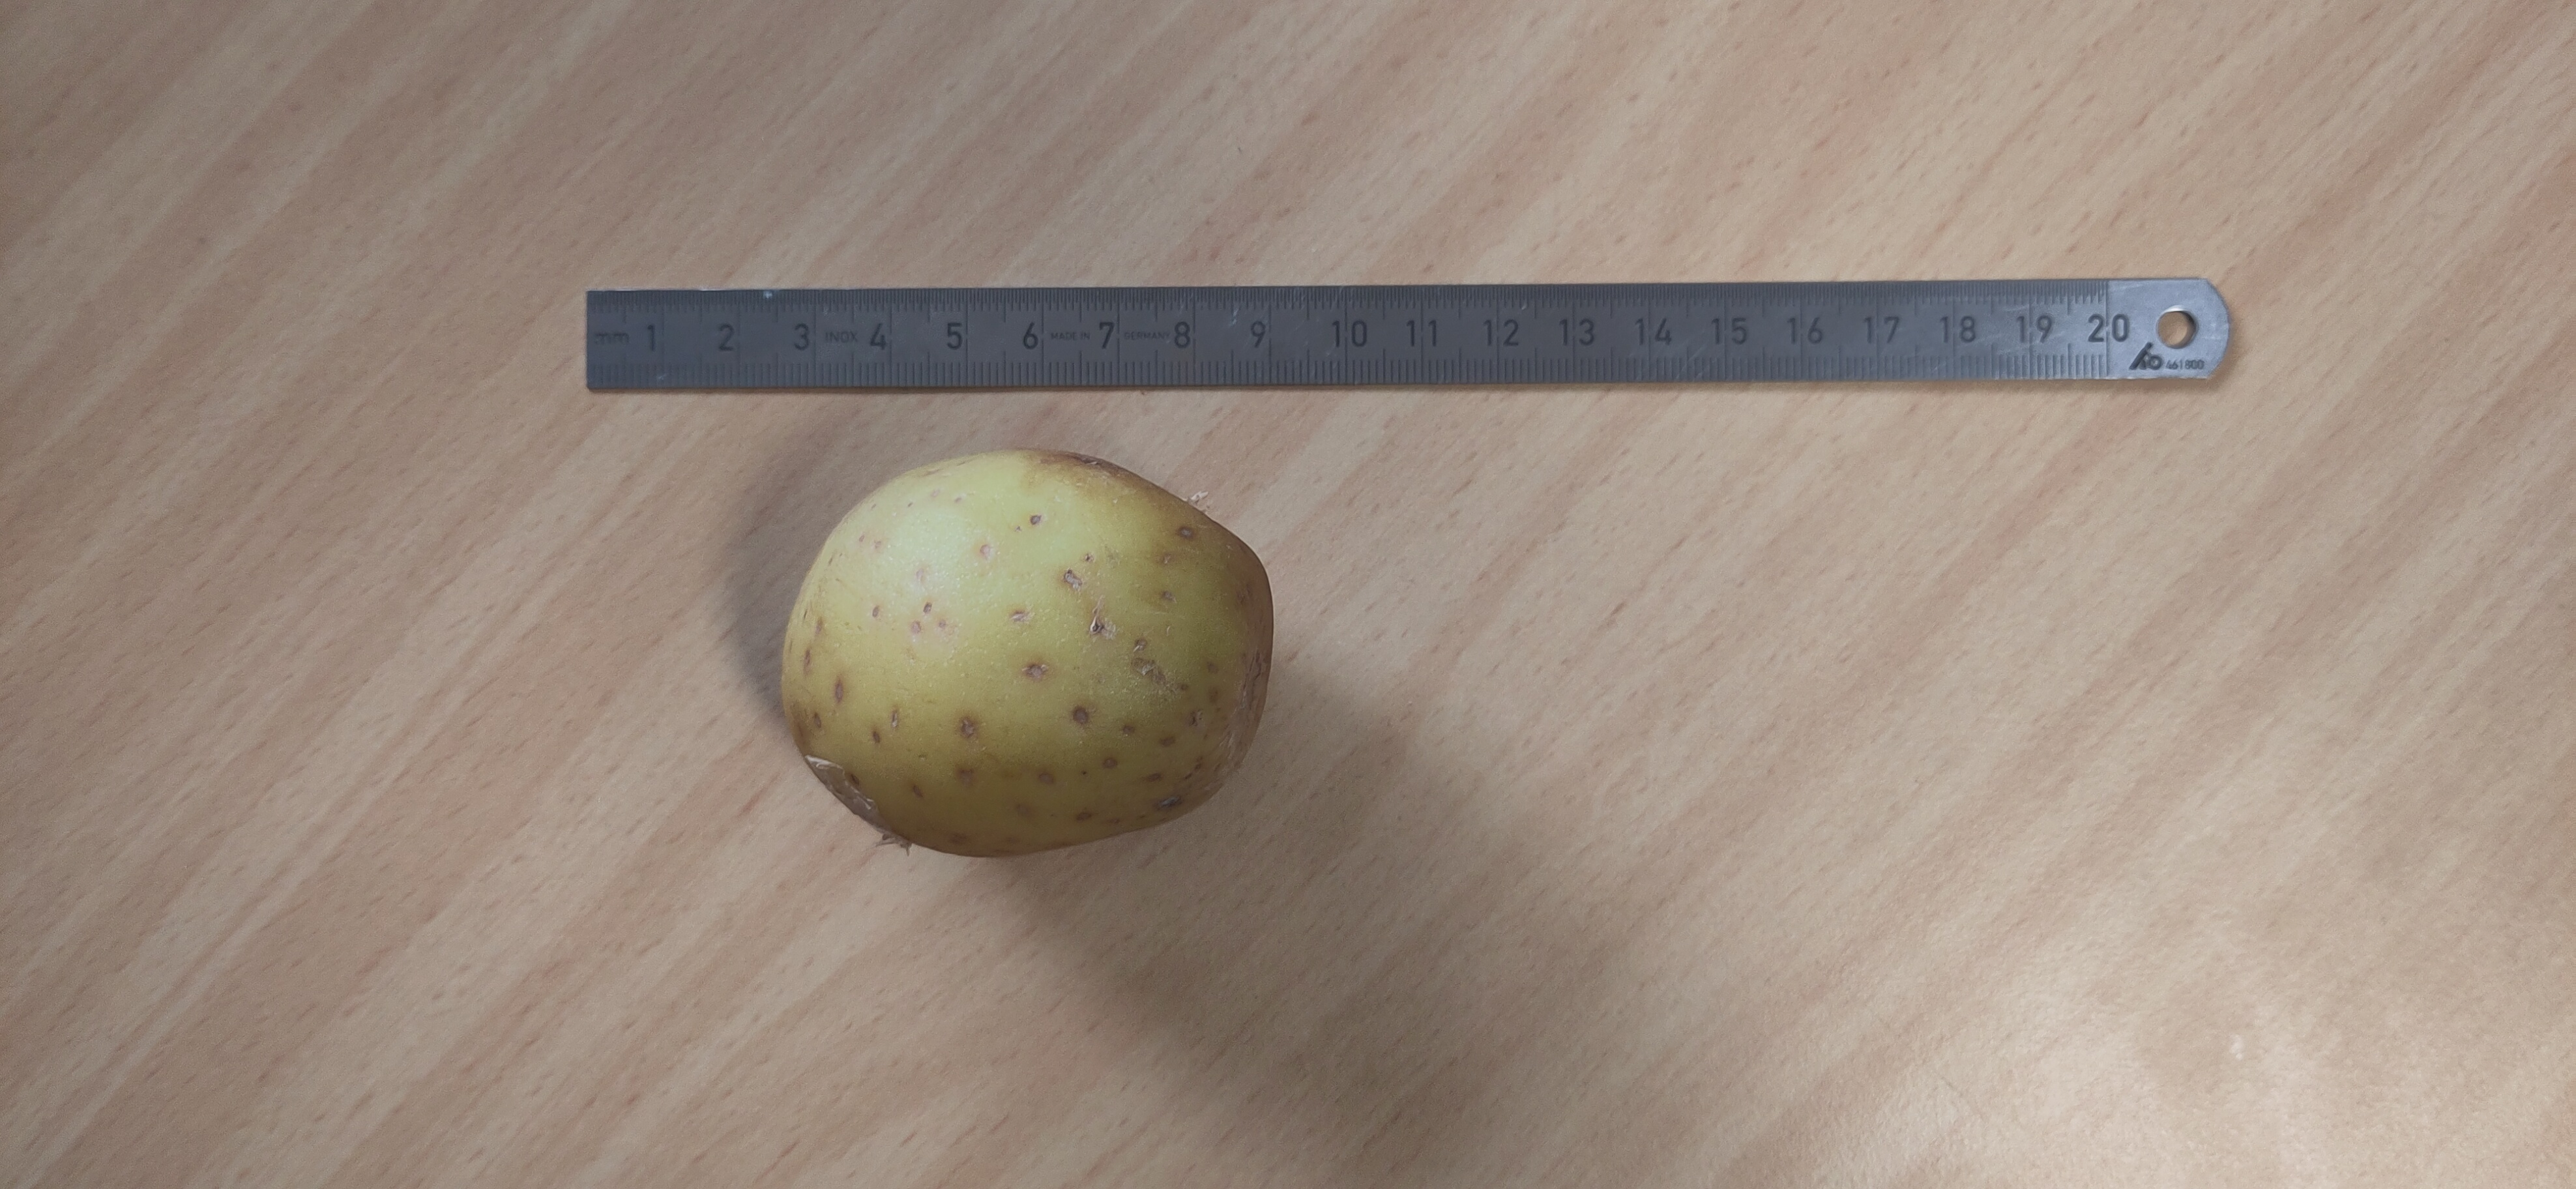
\includegraphics[width=0.8\textwidth]{images/image_2.jpg}
			\vspace{0.2em}
			
			\textbf{Verdächtiges Bild:}
			\vspace{0.3em}
			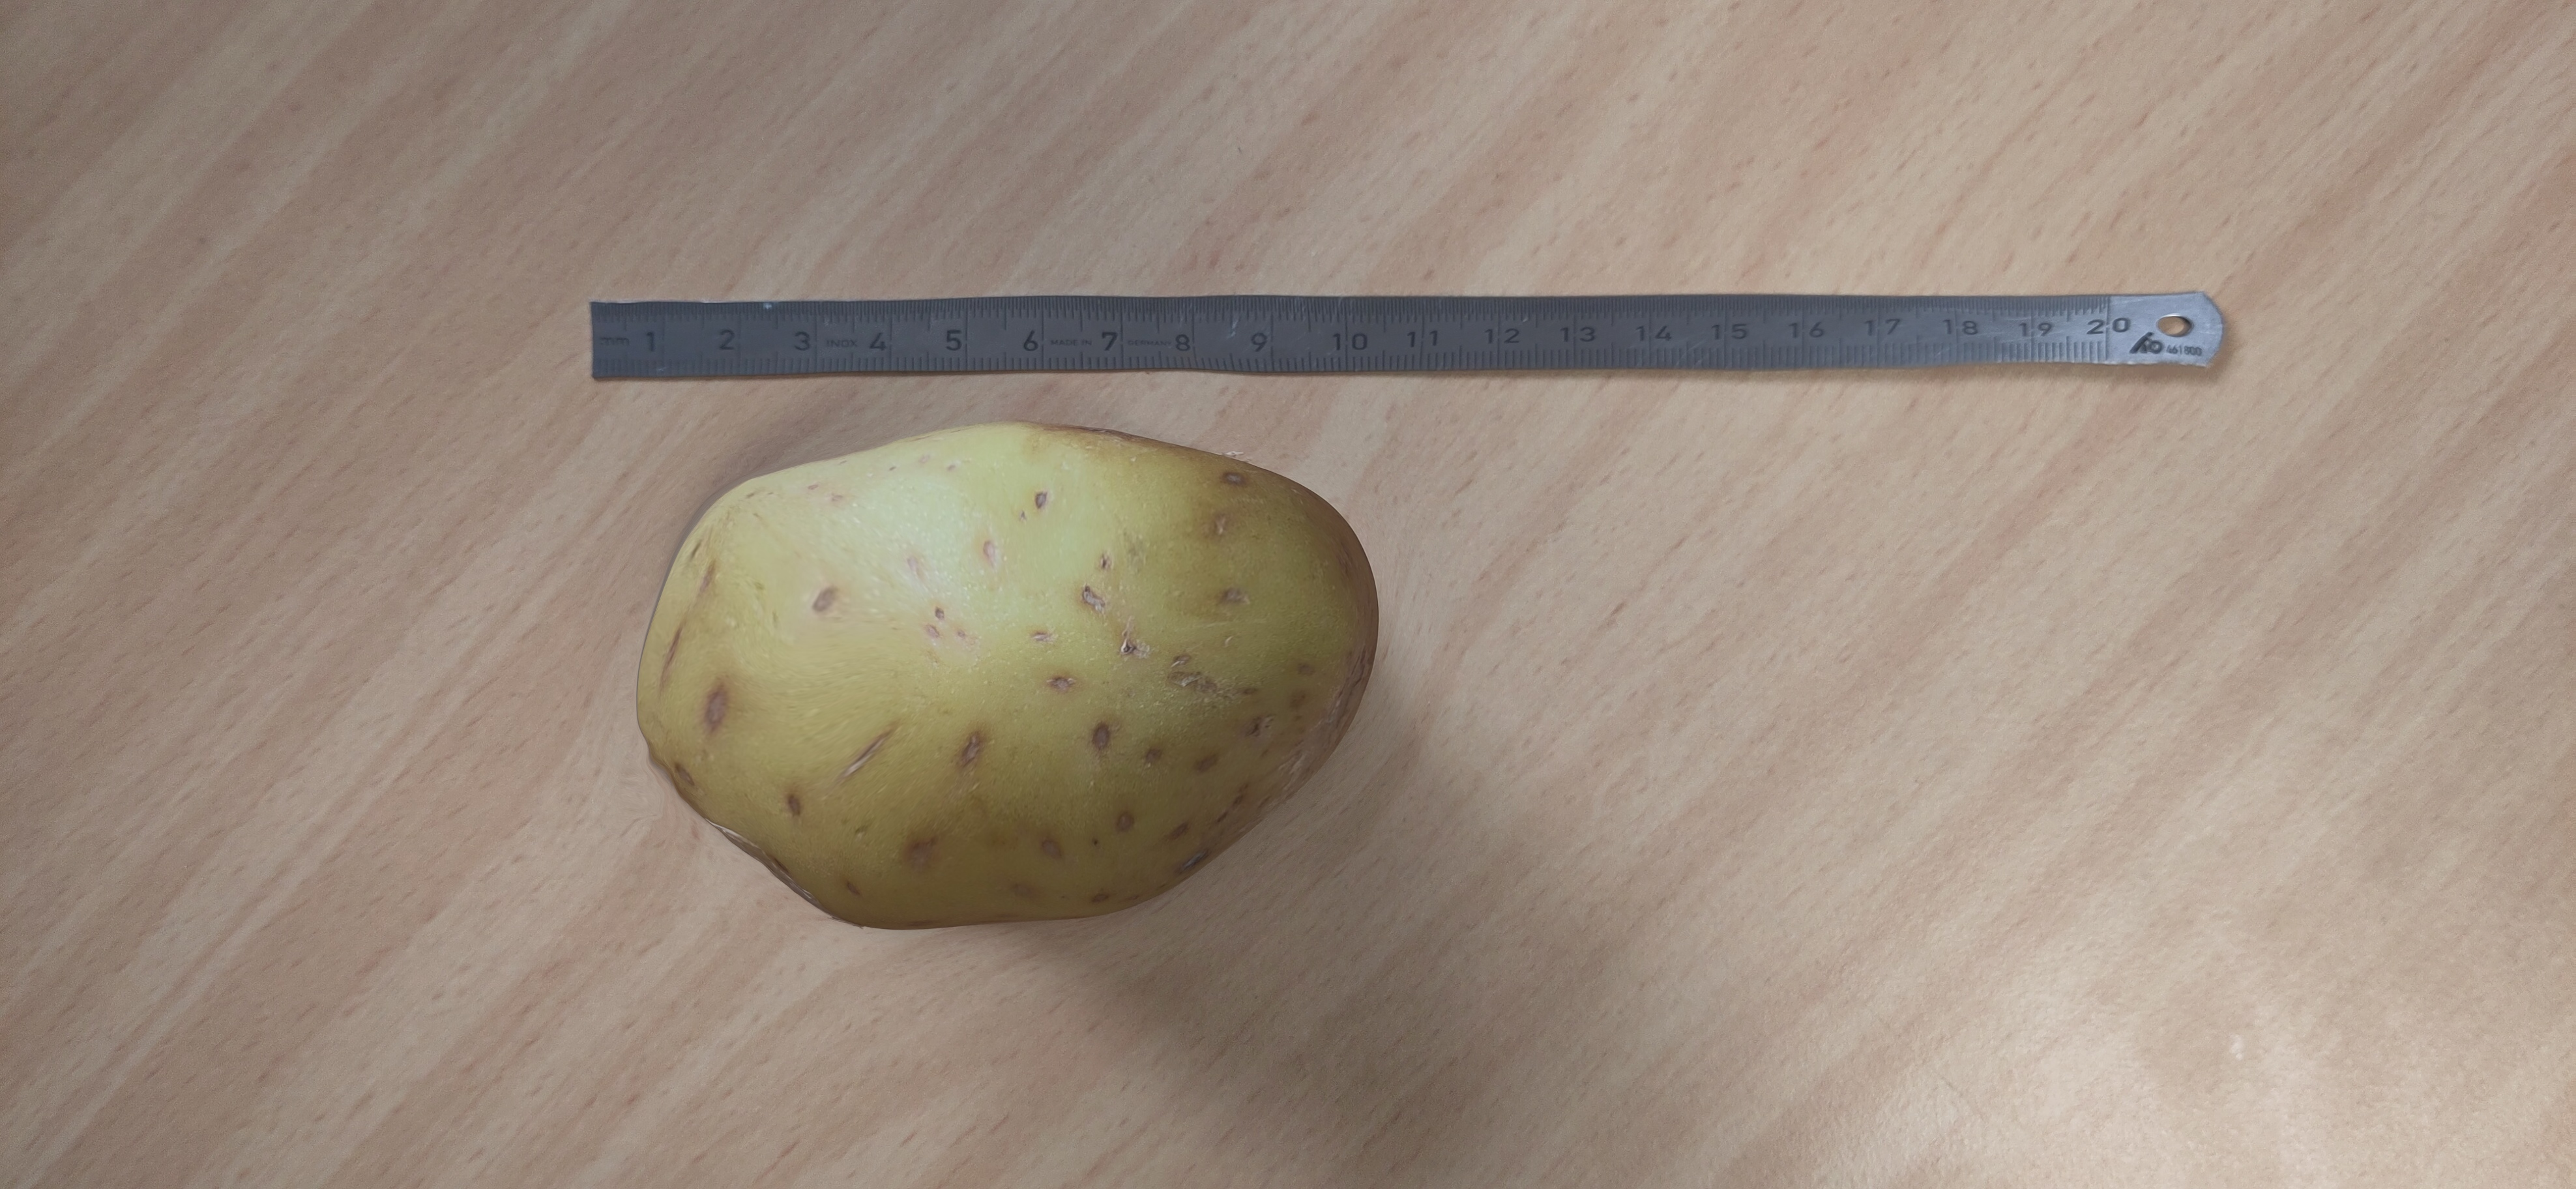
\includegraphics[width=0.8\textwidth]{images/image_2_s.jpg}
			\vspace{0.2em}
		\end{column}
	\end{columns}
\end{frame}


\subsection{Kirchner's Fast Detection Method}

\begin{frame}
	\frametitle{Interpolations-Methoden: Einfache Algorithmen}
	
	\begin{columns}[T]
		\begin{column}{0.48\textwidth}
			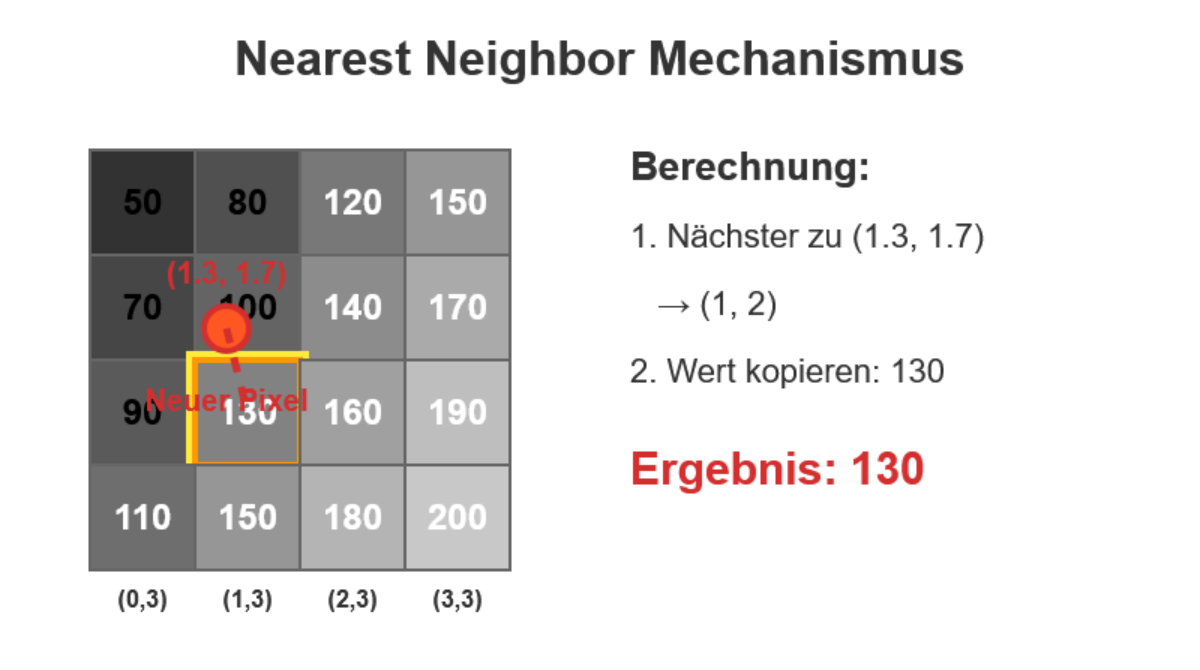
\includegraphics[width=\textwidth]{images/nearest_mechanism.png}
			\textcolor{blue}{\small Blockige Kanten, keine Glättung}\footnote{\tiny Bild mit Hilfe von KI erstellt}
		\end{column}
		\begin{column}{0.48\textwidth}
			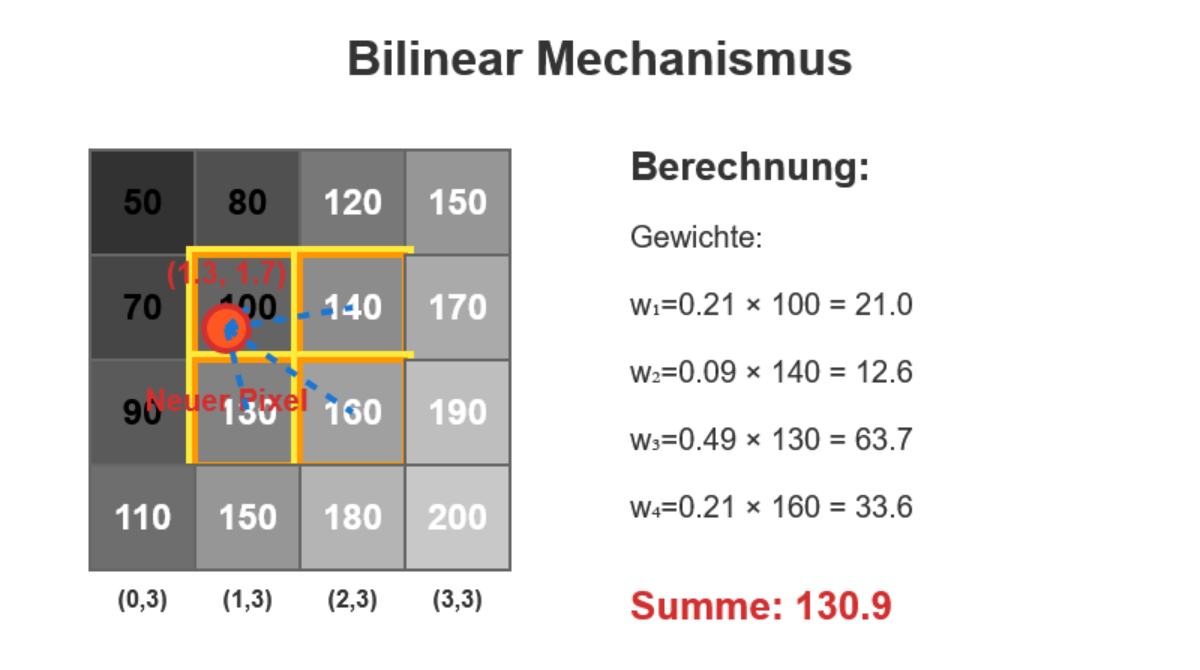
\includegraphics[width=\textwidth]{images/bilinear_mechanism.png}
			\textcolor{blue}{\small Glatte Übergänge, leichte Unschärfe}\footnote{\tiny Bild mit Hilfe von KI erstellt}
		\end{column}
	\end{columns}
	
	\begin{alertblock}{Detektierbarkeit}
		\textcolor{green}{\textbf{Einfach zu detektieren}} - erzeugen starke periodische Muster
	\end{alertblock}
\end{frame}

\begin{frame}
	\frametitle{Interpolations-Methoden: Fortg. Algorithmen}
	
	\begin{columns}[T]
		\begin{column}{0.48\textwidth}
			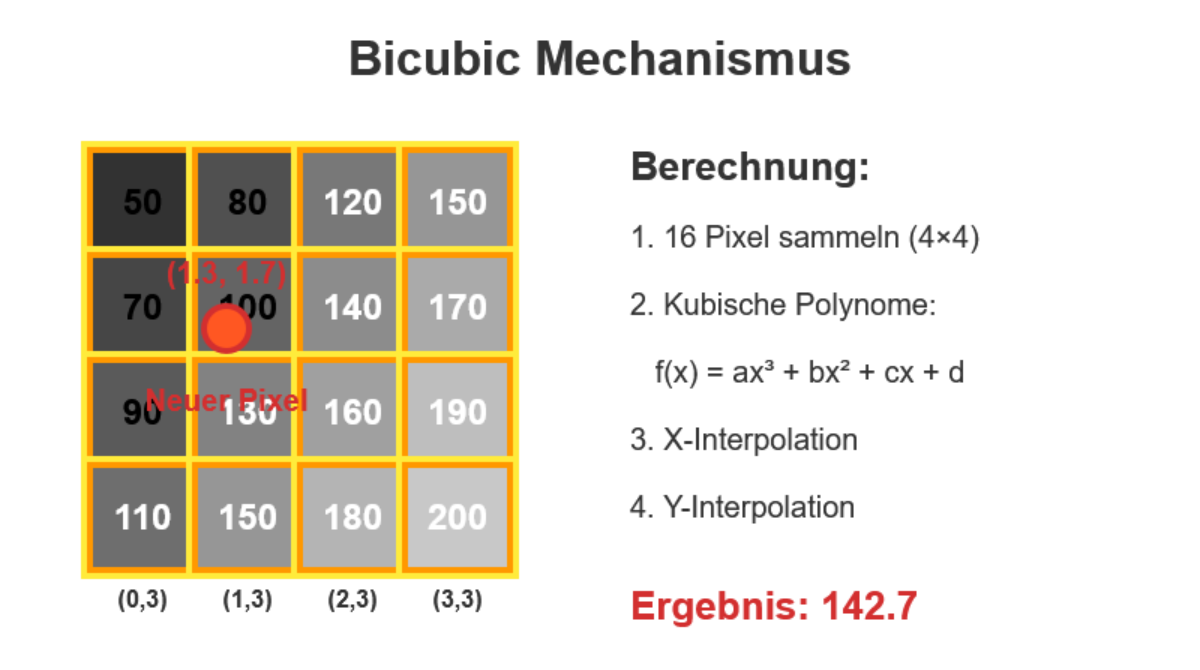
\includegraphics[width=\textwidth]{images/bicubic_mechanism.png}
			\textcolor{blue}{\small Sehr glatt, hochwertige Qualität}\footnote{\tiny Bild mit Hilfe von KI erstellt}
		\end{column}
		\begin{column}{0.48\textwidth}
			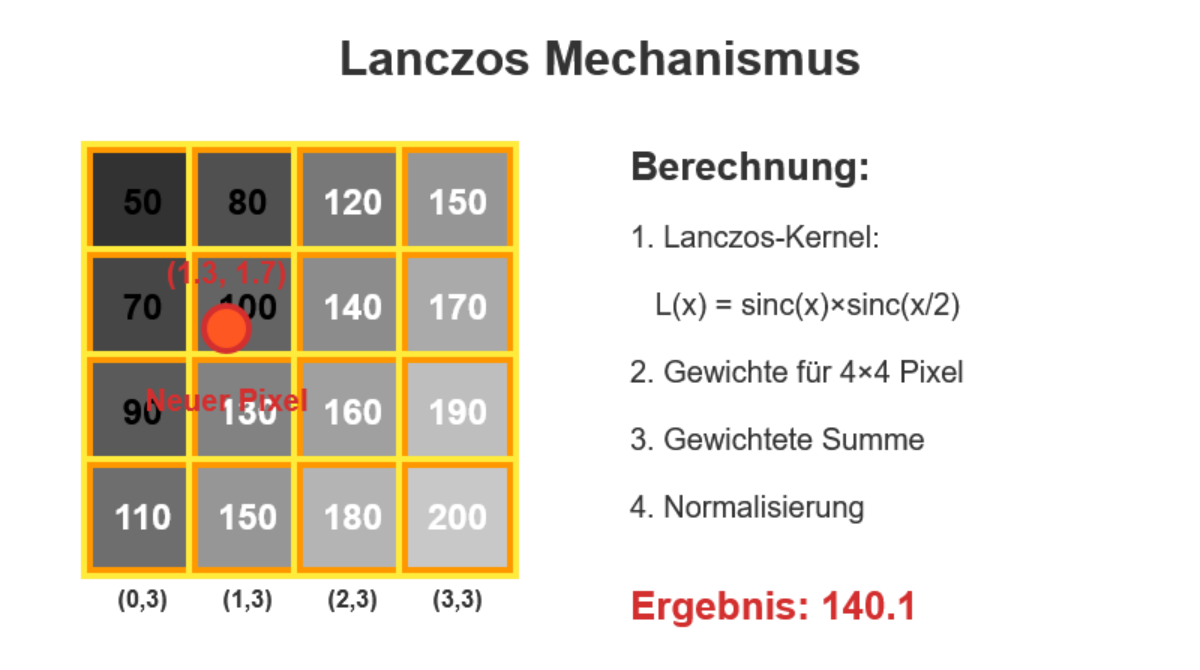
\includegraphics[width=\textwidth]{images/lanczos_mechanism.png}
			\textcolor{blue}{\small Schärfste Details, komplexer Algorithmus}\footnote{\tiny Bild mit Hilfe von KI erstellt}
		\end{column}
	\end{columns}
	
	\begin{alertblock}{Detektierbarkeit}
		\textcolor{red}{\textbf{Schwieriger zu detektieren}} - subtilere periodische Muster
	\end{alertblock}
\end{frame}

\begin{frame}
	\frametitle{Das "Rezept": Kirchner's Fast Detection (2008)}
	
	\begin{exampleblock}{Warum Kirchner's Methode?}
		\begin{itemize}
			\item 40x schneller als Popescu \& Farid~\cite{popescu_exposing_2005}
			\item Keine komplexe EM-Iteration notwendig
			\item Feste Filter-Koeffizienten
			\item Vergleichbare Genauigkeit
		\end{itemize}
	\end{exampleblock}
	
	\vspace{0.5em}
	
	\textbf{Grundprinzip:}
	\begin{enumerate}
		\item \textbf{Input:} Verdächtiges Bild
		\item \textbf{Prozess:} Suche nach periodischen Interpolations-Artefakten
		\item \textbf{Output:} Klassifikation als "Resampled" oder "Original"
	\end{enumerate}
\end{frame}

\begin{frame}
	\frametitle{Schritt 1: Linear Prediction Filter}
	
	\begin{columns}[T]
		\begin{column}{0.45\textwidth}
			\textbf{Filter-Koeffizienten (fest):}
			\vspace{0.5em}
			
			$$\alpha^* = \begin{bmatrix} 
			-0.25 & 0.50 & -0.25 \\
			0.50 & 0 & 0.50 \\
			-0.25 & 0.50 & -0.25
			\end{bmatrix}$$
			
			\vspace{0.5em}
			\textbf{Prediction Error:}
			$$e(i,j) = p(i,j) - \sum_{k,l} \alpha^*_{k,l} \cdot p(i+k,j+l)$$
		\end{column}
		\begin{column}{0.5\textwidth}
			\textbf{Was passiert hier?}
			\begin{itemize}
				\item Jeder Pixel wird durch Nachbarn vorhergesagt
			\end{itemize}
			
			\vspace{0.5em}
			\textbf{Warum feste Koeffizienten?}
			\begin{itemize}
				\item Interpolation erzeugt periodische Artefakte \textit{unabhängig} von den exakten Koeffizienten
				\item Massive Beschleunigung(im vergleich zu EM)
			\end{itemize}
		\end{column}
	\end{columns}
\end{frame}

\begin{frame}
	\begin{columns}[T]
		\begin{column}{0.60\textwidth}
			\frametitle{Schritt 1: Linear Prediction Filter - How it works~\footnote{\textit{Anmerkung:} Stark Simplifiziert, um Konzept zu verdeutlichen}}
			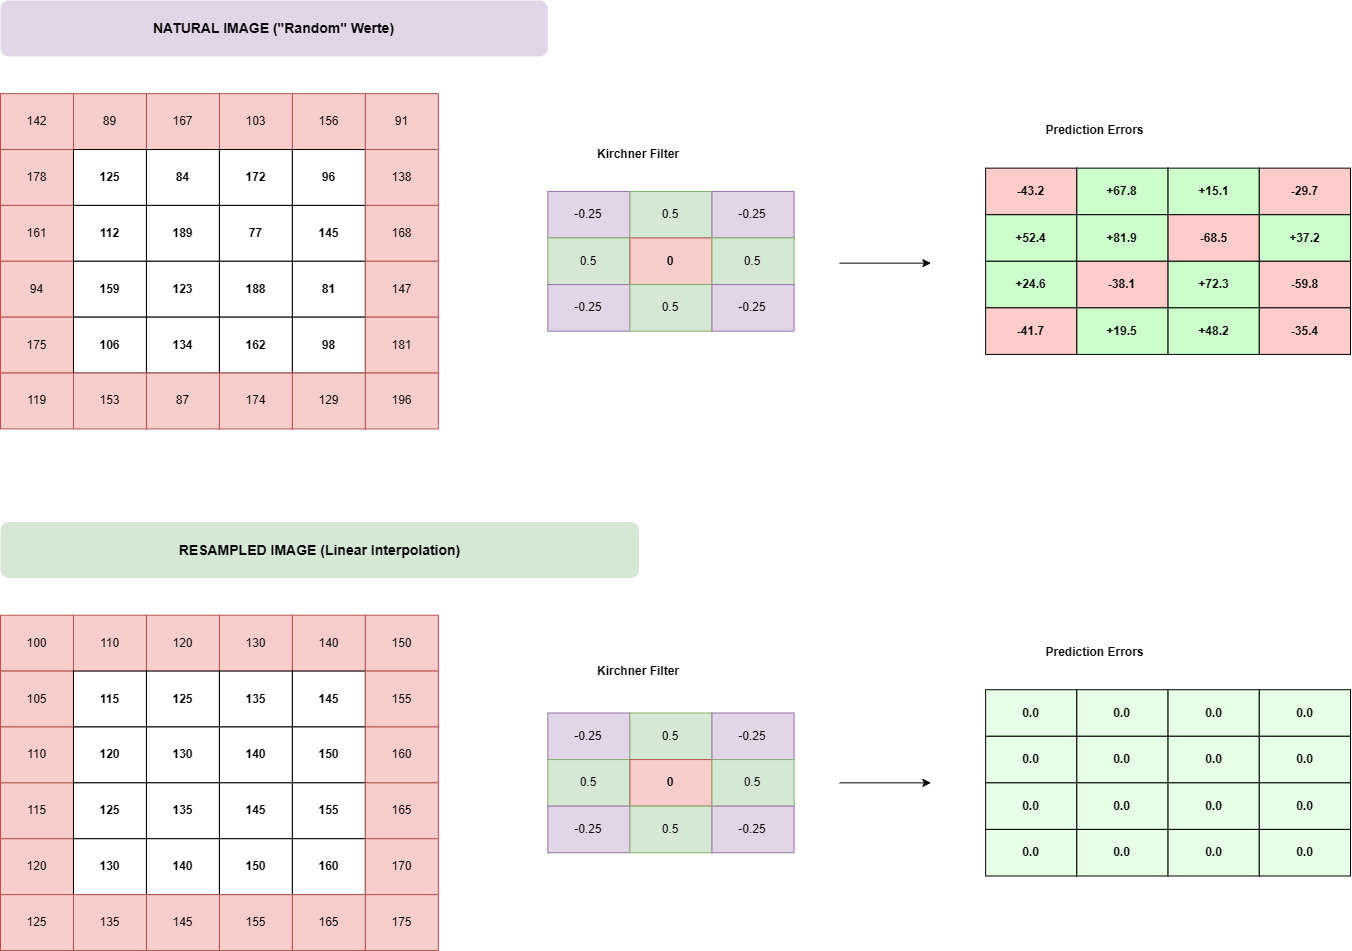
\includegraphics[width=\textwidth]{images/apply_filter.png}
		\end{column}
		\begin{column}{0.38\textwidth}
			\begin{itemize}
				\item \textcolor{blue}{Vorhersagefehler} wird für jedes Pixel berechnet
				\item \textcolor{blue}{Periodische Muster} erzeugen starke Korrelationen
			\end{itemize}
		\end{column}			
	\end{columns}

\end{frame}

\begin{frame}
	\frametitle{Schritt 1: Linear Prediction Filter - Visualisierung}
	\begin{columns}[T]
		\begin{column}{0.48\textwidth}
			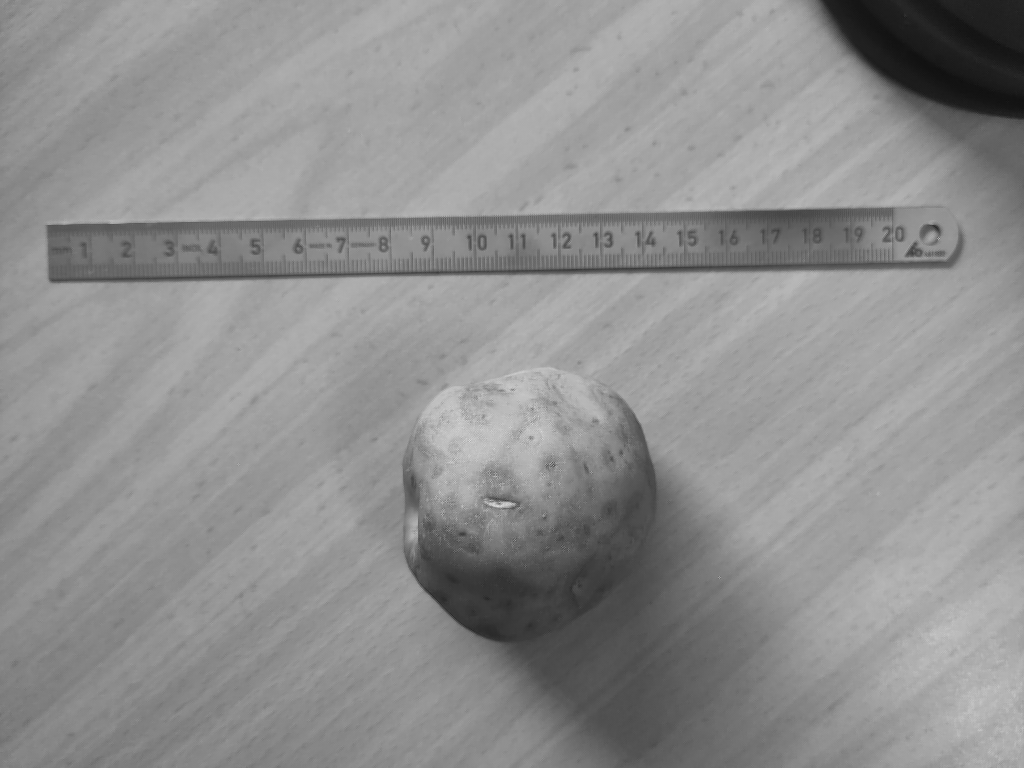
\includegraphics[width=\textwidth]{images/examples_unedited/predicted.png}
			\textcolor{green}{\small Original Prediction Error}
		\end{column}
		\begin{column}{0.48\textwidth}
			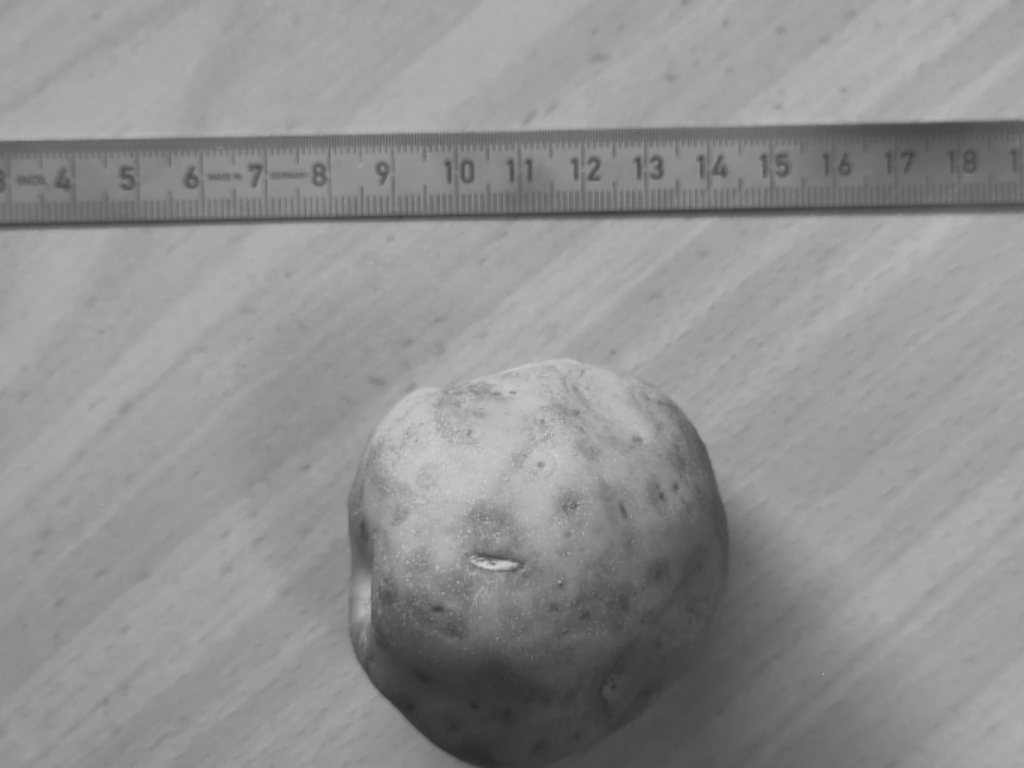
\includegraphics[width=\textwidth]{images/examples_edited/predicted.png}
			\textcolor{red}{\small Resampled Prediction Error}
		\end{column}
	\end{columns}
\end{frame}

\begin{frame}
	\frametitle{Schritt 1: Linear Prediction Filter - Visualisierung}
	
	\begin{columns}[T]
		\begin{column}{0.48\textwidth}
			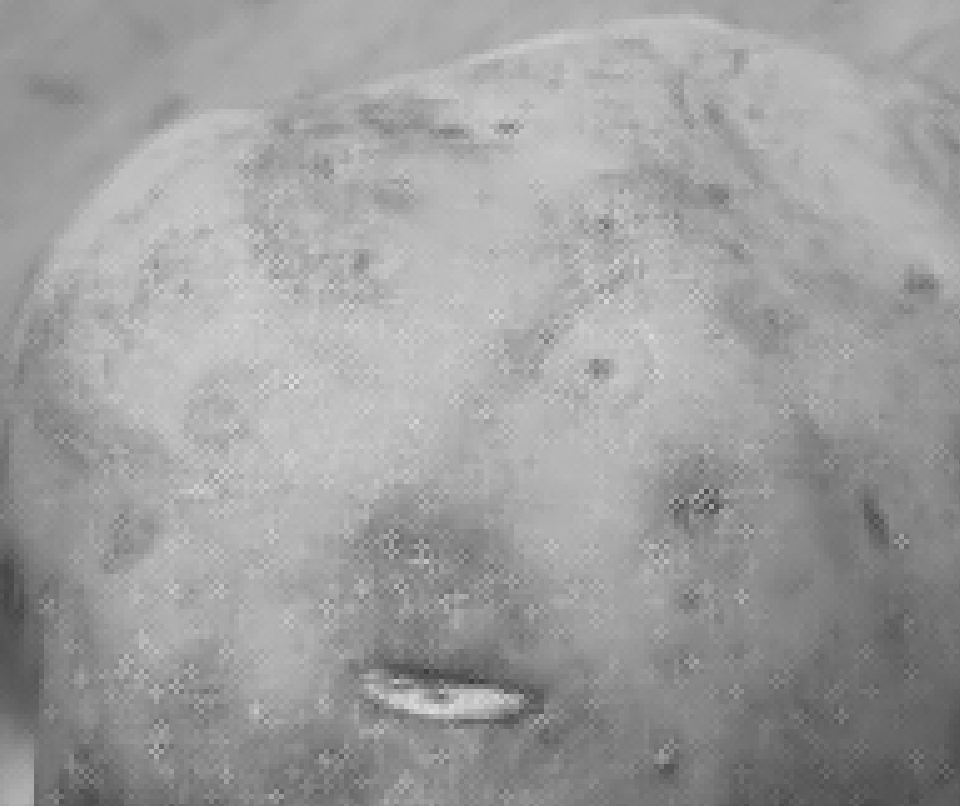
\includegraphics[width=\textwidth]{images/examples_unedited/predicted_zoom.png}
			\textcolor{green}{\small Original Prediction Error}
		\end{column}
		\begin{column}{0.48\textwidth}
			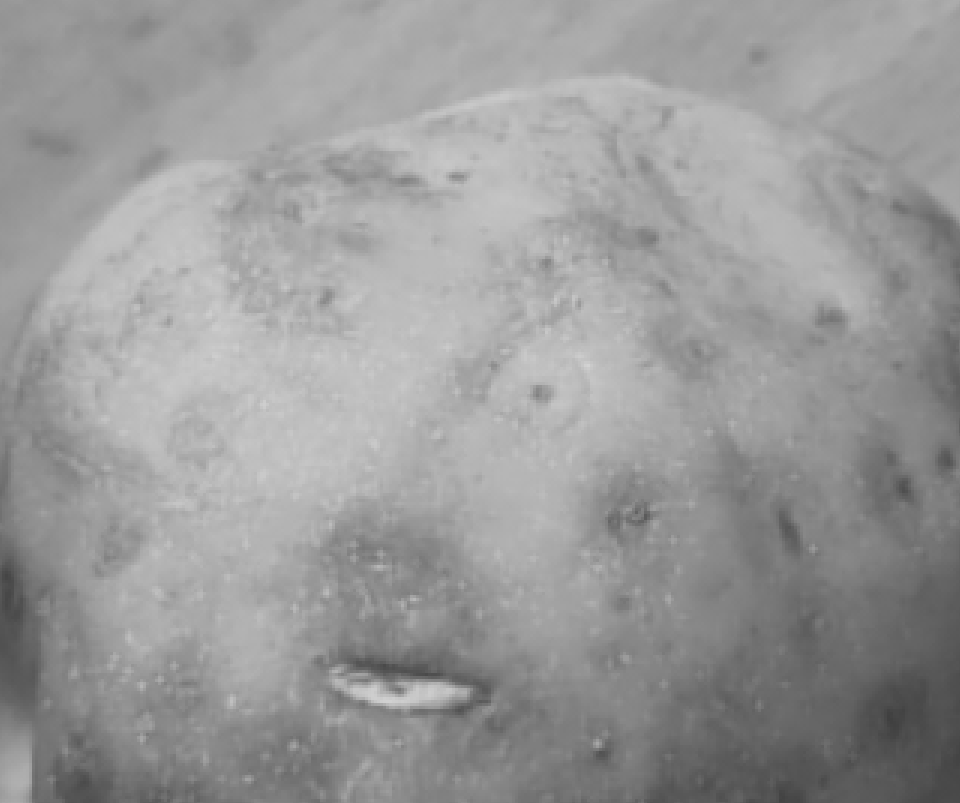
\includegraphics[width=\textwidth]{images/examples_edited/predicted_zoom.png}
			\textcolor{red}{\small Resampled Prediction Error}
		\end{column}
	\end{columns}
\end{frame}

\begin{frame}
	\frametitle{Schritt 2: P-Map Generation}
	
	\begin{columns}[T]
		\begin{column}{0.45\textwidth}
			\textbf{Contrast Function:}
			$$p(i,j) = \lambda \cdot \exp\left(-\frac{|e(i,j)|^\tau}{\sigma}\right)$$
			
			\vspace{0.5em}
			\textbf{Parameter:}
			\begin{itemize}
				\item $\lambda = 1$ (Normalisierung)
				\item $\sigma = 1$ (Schwellwert)
				\item $\tau = 2$ (Kontrast-Exponent)
			\end{itemize}
		\end{column}
		\begin{column}{0.5\textwidth}
			\textbf{Was macht die P-Map?}
			\begin{itemize}
				\item \textcolor{blue}{Kleine Errors} → Hohe P-Map Werte
				\item \textcolor{red}{Große Errors} → Niedrige P-Map Werte
				\item Verstärkt periodische Muster
			\end{itemize}
			
			\vspace{0.5em}
			\textbf{Ergebnis:}
			\begin{itemize}
				\item Interpolierte Bereiche zeigen periodische P-Map
				\item Echte Bereiche zeigen zufällige P-Map
			\end{itemize}
		\end{column}
	\end{columns}
\end{frame}

\begin{frame}
	\frametitle{Schritt 2: P-Map Generation - Visualisierung}

	\begin{columns}[T]
		\begin{column}{0.48\textwidth}
			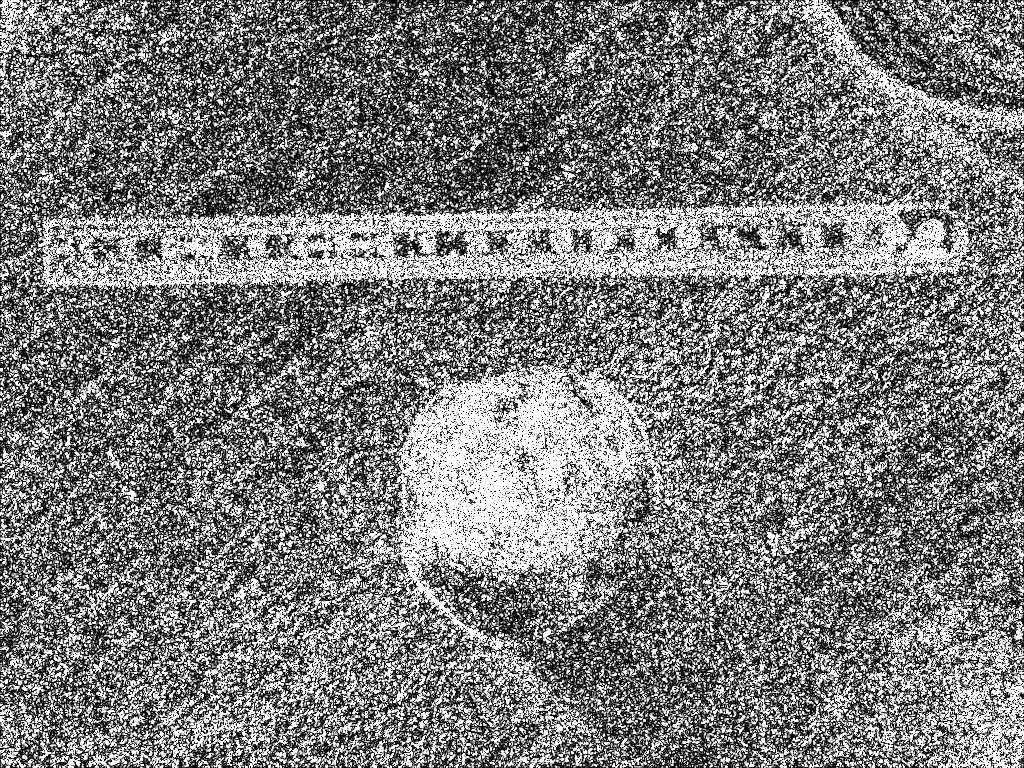
\includegraphics[width=\textwidth]{images/examples_unedited/p_map.png}
			\textcolor{green}{\small Original P-Map (Zufällig)}
		\end{column}
		\begin{column}{0.48\textwidth}
			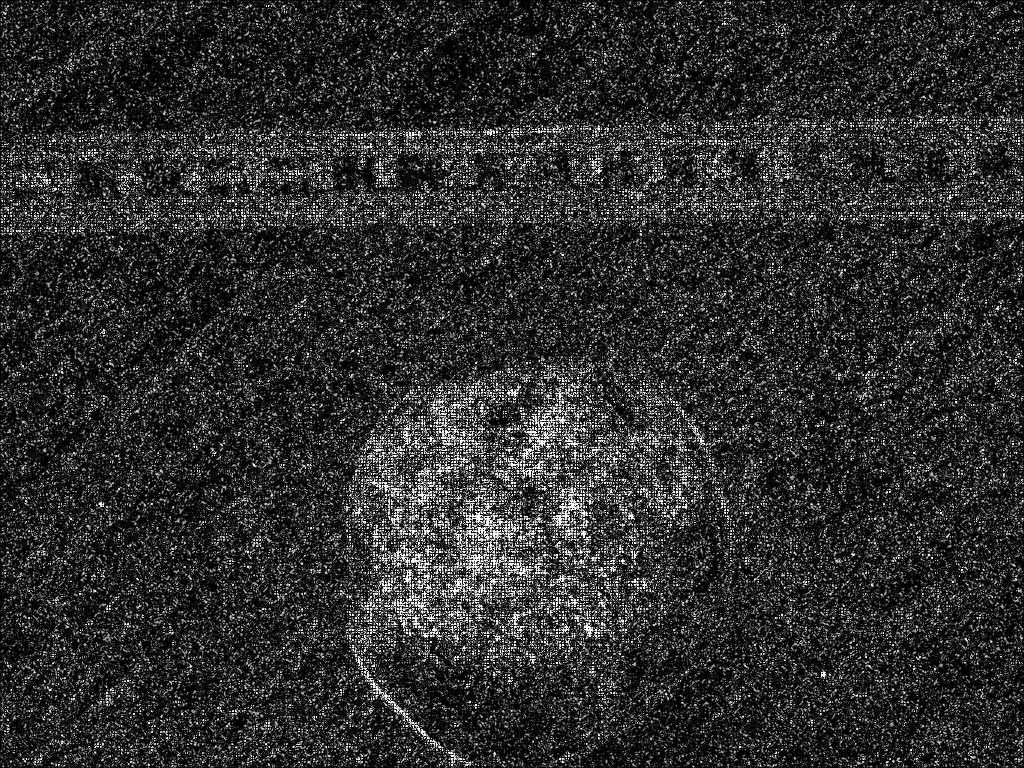
\includegraphics[width=\textwidth]{images/examples_edited/p_map.png}
			\textcolor{red}{\small Resampled P-Map (Periodisch)}
		\end{column}
	\end{columns}
\end{frame}

\begin{frame}
	\frametitle{Schritt 2: P-Map Generation - Visualisierung}
	
	\begin{columns}[T]
		\begin{column}{0.48\textwidth}
			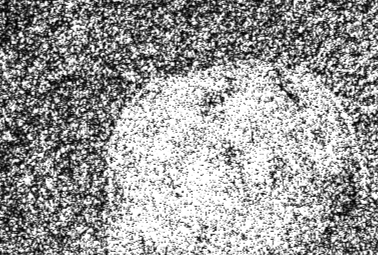
\includegraphics[width=\textwidth]{images/examples_unedited/p_map_zoom.png}
			\textcolor{green}{\small Original P-Map (Zufällig)}
		\end{column}
		\begin{column}{0.48\textwidth}
			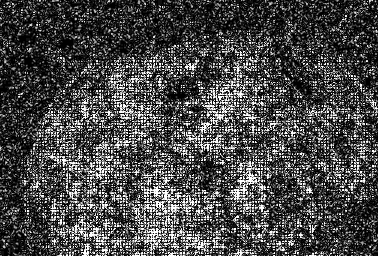
\includegraphics[width=\textwidth]{images/examples_edited/p_map_zoom.png}
			\textcolor{red}{\small Resampled P-Map (Periodisch)}
		\end{column}
	\end{columns}
\end{frame}

\begin{frame}
	\frametitle{Schritt 3: Spektralanalyse \& Peak Detection}
	
	\begin{columns}[T]
		\begin{column}{0.45\textwidth}
			\textbf{Fourier Transform:}
			$$P_f = \text{DFT}(p)$$
			
			\vspace{0.5em}
			\textbf{Cumulative Periodogram:}
			$$C(f) = \frac{\sum_{0<f' \leq f} |P(f')|^2}{\sum_{0<f' \leq f_{max}} |P(f')|^2}$$
			
			\vspace{0.5em}
			\textbf{Decision Criterion:}
			$$\delta' = \max_f |\nabla C(f)|$$
		\end{column}
		\begin{column}{0.5\textwidth}
			\textbf{Peak Detection Logic:}
			\begin{itemize}
				\item \textcolor{blue}{Periodische P-Map} → Scharfe Peaks im Spektrum
				\item \textcolor{blue}{Zufällige P-Map} → Gleichmäßiges Spektrum
			\end{itemize}
			
			\vspace{0.5em}
			\textbf{Automatische Detektion:}
			\begin{itemize}
				\item Maximum des Gradienten im Cumulative Periodogram
				\item Schwellwert $\delta'_T$ für Klassifikation
				\item \textcolor{green}{$\delta' > \delta'_T$} → Resampled
				\item \textcolor{red}{$\delta' \leq \delta'_T$} → Original
			\end{itemize}
		\end{column}
	\end{columns}
\end{frame}

\begin{frame}
	\frametitle{Schritt 3: Spektralanalyse - Visualisierung}
	
	\begin{columns}[T]
		\begin{column}{0.48\textwidth}
			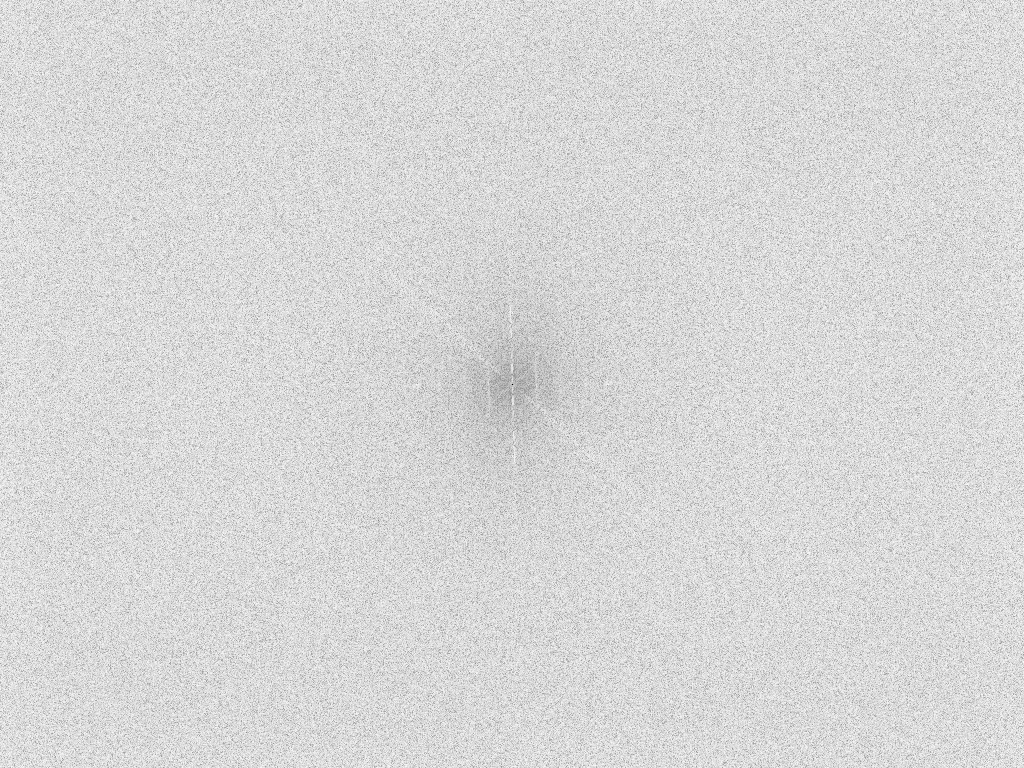
\includegraphics[width=\textwidth]{images/examples_unedited/spectrum.png}
			\textcolor{green}{\small Original Spektrum (Zufällig)}
		\end{column}
		\begin{column}{0.48\textwidth}
			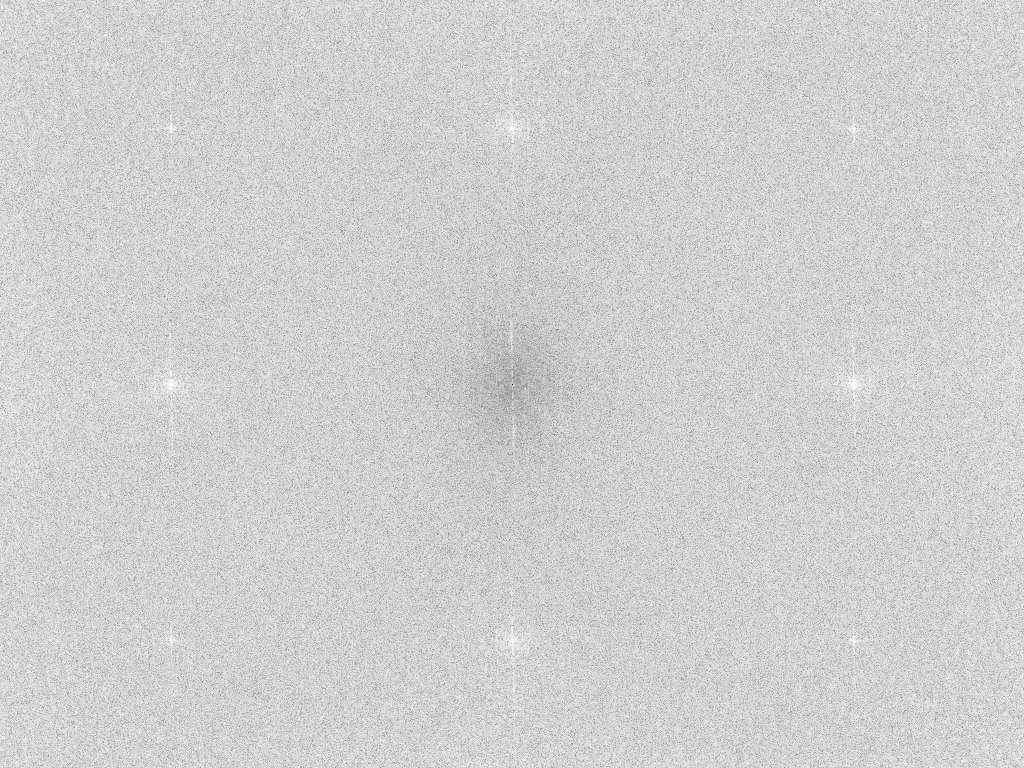
\includegraphics[width=\textwidth]{images/examples_edited/spectrum.png}
			\textcolor{red}{\small Resampled Spektrum (Periodisch)}
		\end{column}
	\end{columns}
\end{frame}

\begin{frame}
	\frametitle{Schritt 3: Decision Criterion - Visualisierung}
	\begin{columns}[T]
		\begin{column}{0.48\textwidth}
			
\includegraphics[width=\textwidth]{images/examples_unedited/gradient_map.png}
			\textcolor{green}{\small Original Gradienten Map("Zufällig")}
		\end{column}
		\begin{column}{0.48\textwidth}
			
\includegraphics[width=\textwidth]{images/examples_edited/gradient_map.png}
			\textcolor{red}{\small Resampled Gradienten Map("Periodisch")}
		\end{column}
	\end{columns}
\end{frame}

\subsection{Praktische Anwendung}

\begin{frame}
	\frametitle{Fallauflösung: Analyseergebnisse}
	\begin{columns}[T]
		\begin{column}{0.6\textwidth}
			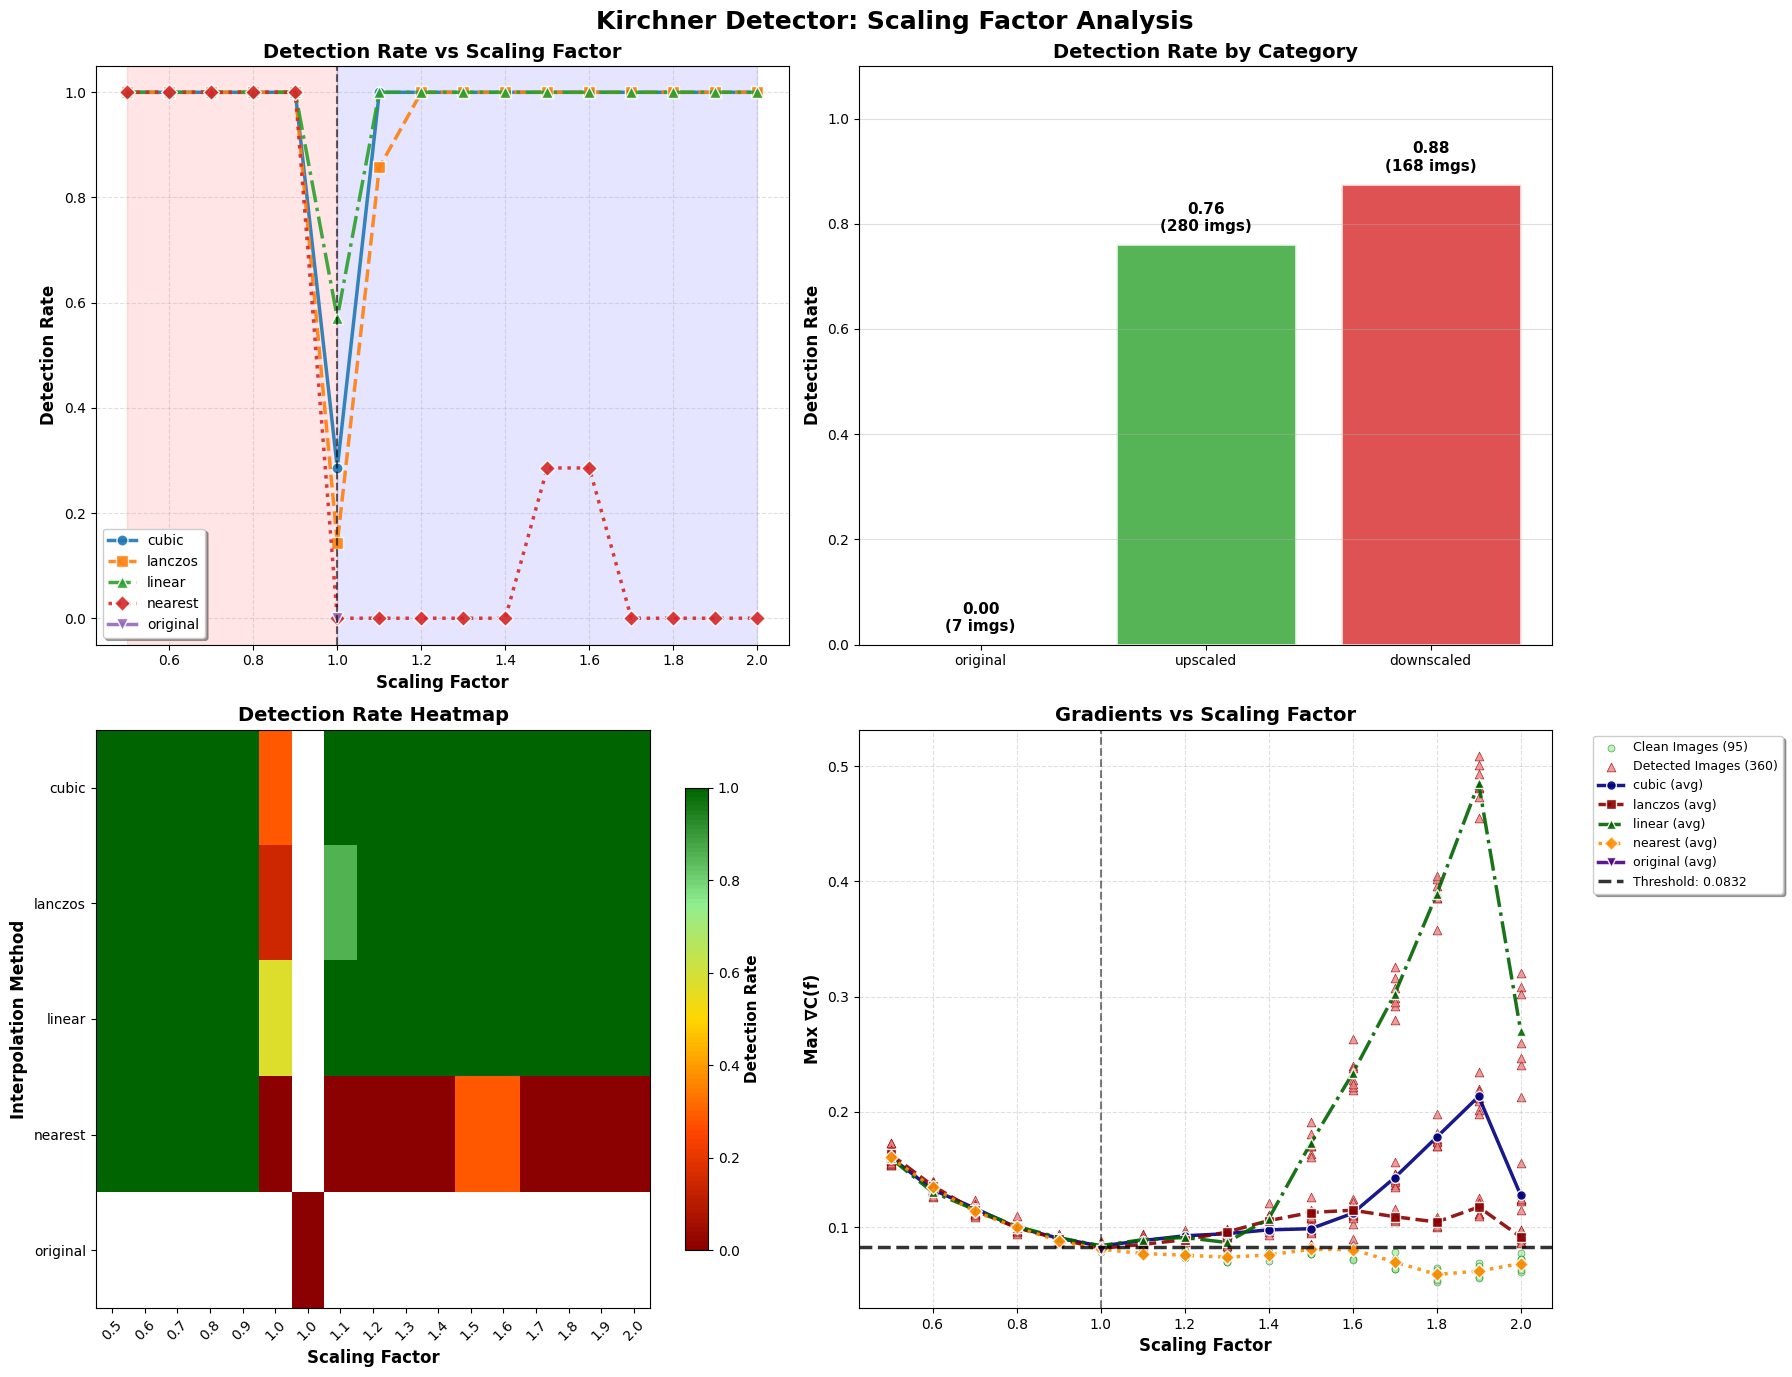
\includegraphics[width=\textwidth]{images/scaling_analysis_report.png}
		\end{column}
		\begin{column}{0.40\textwidth}
			\begin{itemize}
				\item 11 Originalbilder
				\item 10 Scalierungsfaktoren(110 Bilder)
			\end{itemize}
		\end{column}
	\end{columns}
\end{frame}

\begin{frame}
	\frametitle{Fallauflösung: Analyseergebnisse}
	\begin{columns}[T]
		\begin{column}{0.6\textwidth}
			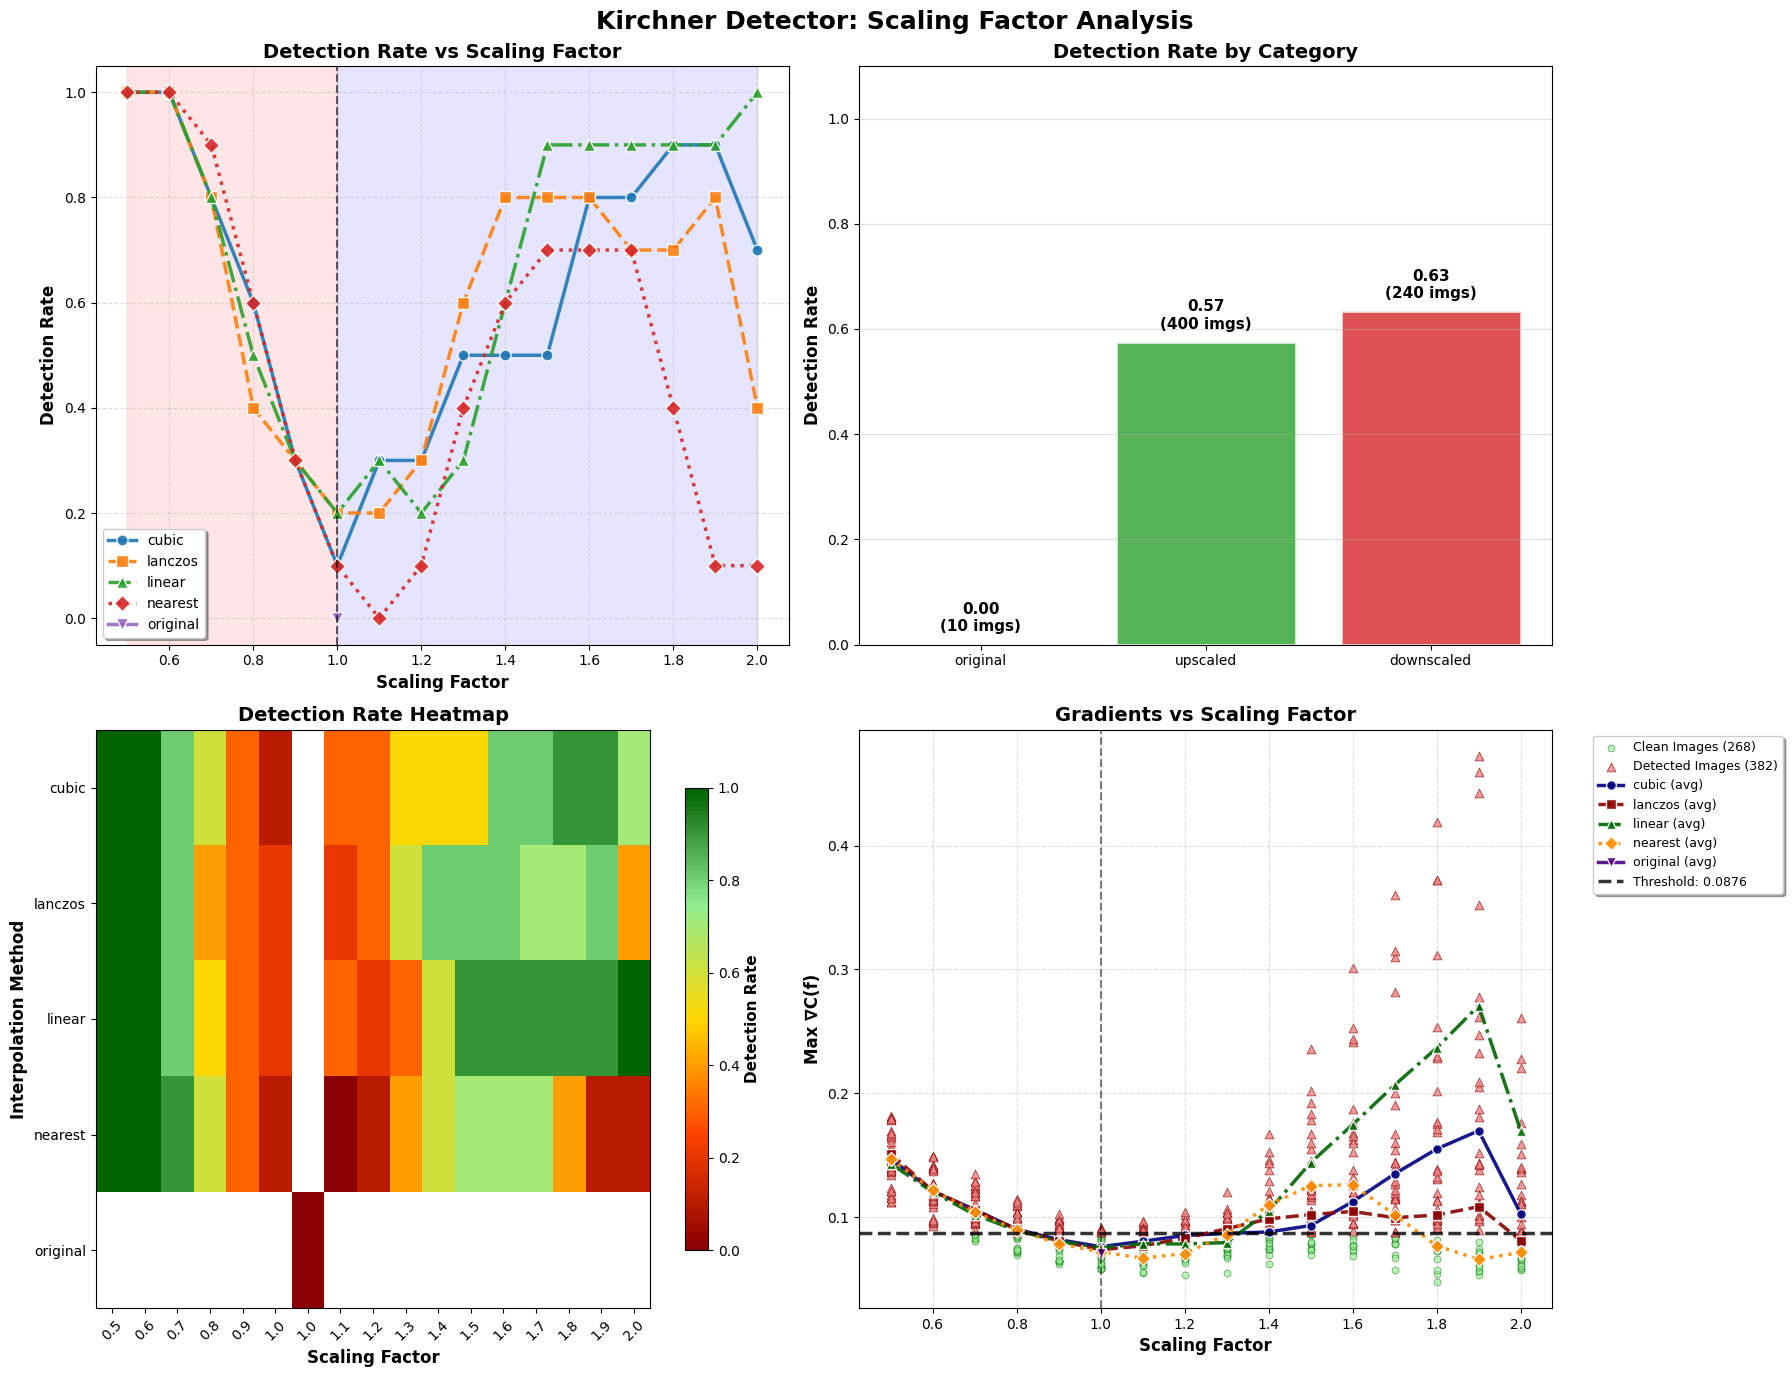
\includegraphics[width=\textwidth]{images/scaling_analysis_report_full.png}
		\end{column}
		\begin{column}{0.40\textwidth}
			\begin{itemize}
				\item 11 Originalbilder
				\item 10 Scalierungsfaktoren(110 Bilder)
				\item 4 Interpolationsmethoden(451 Bilder)
			\end{itemize}
		\end{column}
	\end{columns}
\end{frame}

\subsection{Grenzen \& Lessons Learned}

\begin{frame}
	\frametitle{Grenzen der Methode}
	
	\begin{columns}[T]
		\begin{column}{0.48\textwidth}
			\begin{alertblock}{Kritische Einschränkungen}
				\begin{itemize}
					\item \textcolor{red}{Sehr Abhängig vom Bildinhalt} (False Positives)
					\item \textcolor{red}{Fixed Threshold} für $\delta'_T$ kann zu Fehlklassifikationen führen
					\item \textcolor{red}{Interpolationsmethoden} können die Detektion beeinflussen
					\item \textcolor{red}{Anti-Forensik-Methoden} können die Detektion umgehen~\cite{kirchner_hiding_2008}
				\end{itemize}
			\end{alertblock}
		\end{column}
		\begin{column}{0.48\textwidth}
			\begin{exampleblock}{Was funktioniert gut}
				\begin{itemize}
					\item \textcolor{green}{Homogene Bildbereiche, ohne Muster}
				\end{itemize}
			\end{exampleblock}
		\end{column}
	\end{columns}
	
	\vspace{1em}
	
\end{frame}

\begin{frame}
	\frametitle{Fazit \& Praktische Relevanz}
	
	\begin{alertblock}{Praktische Empfehlungen}
		\begin{enumerate}
			\item Verwende multiple forensische Methoden parallel
			\item Prüfe Bildqualität und Kompression vorab
			\item Berücksichtige Bildinhalt (Textur vs. homogene Bereiche)
			\item Interpretiere Ergebnisse als Wahrscheinlichkeiten, nicht Wahrheiten
		\end{enumerate}
	\end{alertblock}
    
    \begin{block}{Lessons Learned}
        \begin{itemize}
            \item Methode ist ein \textbf{Indiz}, kein Beweis
            \item Muss mit anderen forensischen Methoden kombiniert werden
            \item Expertenwissen für Interpretation notwendig
            \item Don't overcomplicate: Einfachheit ist oft effektiver
        \end{itemize}
    \end{block}
\end{frame}

\subsection{Quellen}
\begin{frame}
    \frametitle{Quellen}
    \begingroup
    \setbeamerfont{bibliography item}{size=\tiny}
    \setbeamerfont{bibliography entry author}{size=\tiny}
    \setbeamerfont{bibliography entry title}{size=\tiny}
    \setbeamerfont{bibliography entry location}{size=\tiny}
    \setbeamerfont{bibliography entry note}{size=\tiny}
    \setbeamerfont{bibliography entry year}{size=\tiny}
    \setlength{\bibitemsep}{2pt}
    \setlength{\itemsep}{0pt}
    \setlength{\parskip}{0pt}
    \renewcommand{\bibfont}{\tiny}
    \printbibliography[heading=none]
    \endgroup
\end{frame}

\begin{frame}
	\frametitle{Vielen Dank für Ihre Aufmerksamkeit!}
	
	\vspace{2em}
	
	\begin{center}
		\Large{\textbf{Fragen?}}
		
		\vspace{1.5em}
		
		\textbf{Kirchner's Fast Resampling Detection}
		
		\textit{InterpoLIE-tion - Catching lies through interpolation analysis}
		
		\vspace{1.5em}
		
		\small{Dominik Barbist, Lukas Egger}
	\end{center}
\end{frame}



\end{document}